\documentclass[12pt, a4paper, oneside]{book}

%---------------------------------------------------------   
\usepackage[english,romanian,magyar]{babel}       
\usepackage[utf8]{inputenc}
\usepackage[a4,center,axes]{crop}
\usepackage{calc}
\usepackage{t1enc}
\usepackage{amsthm}
\usepackage{rotating}
\usepackage{amssymb}
\usepackage{lscape}
\usepackage{anysize}
\usepackage{setspace} 
\usepackage{comment}
\usepackage{graphicx}
\usepackage{setspace} 
\usepackage{tocloft}
\usepackage{indentfirst}
\usepackage{url}
\usepackage{listings}
\usepackage[top=3cm, bottom=2cm, left=3cm, right=2cm]{geometry}

%---------------------------------------------------------
%%
%%
%% alapformázások
%%
%%
\sloppy                        % sorkizárás kezelése
\clubpenalty = 10000           % árvasorok
\widowpenalty = 10000          % fatyúsorok
\raggedbottom                  % függõleges kizárás az oldalon
\setcounter{secnumdepth}{3}    % alcimek számozási mélysége
\setcounter{tocdepth}{3}       % tartalomjegyzék mélysége
\brokenpenalty = 10000         % lap aljai elválasztások tiltása
\doublehyphendemerits = 80000  % egymást követõ elválasztások

%\marginsize{2cm}{2cm}{2cm}{2cm} %marók beállítása
\onehalfspacing %sorközök megaddása

\theoremstyle{tetel}
\newtheorem{mydef}{értelmezés}[chapter]
\newtheorem{megj}{megjegyzés}[chapter]

\def\partro#1{\foreignlanguage{romanian}{\addcontentsline{tro}{part}{%\if@mainmatter\protect\numberline{\thechapter.}\fi
\MakeUppercase{#1}}}}
\def\chapterro#1{\foreignlanguage{romanian}{\addcontentsline{tro}{chapter}{\if@mainmatter\protect\numberline{\thechapter.}\fi#1}}}
\def\sectionro#1{\foreignlanguage{romanian}{\addcontentsline{tro}{section}{\protect\numberline{\thesection.}#1}}}
\def\subsectionro#1{\foreignlanguage{romanian}{\addcontentsline{tro}{subsection}{\protect\numberline{\thesubsection.}#1}}}
\def\subsubsectionro#1{\foreignlanguage{romanian}{\addcontentsline{tro}{subsubsection}{\protect\numberline{\thesubsubsection.}#1}}}

%roman tartalom def
%---------------------------------------------------------
\newcommand{\nombreindice}{Cuprins}
\newlistof{indice}{tce}{\nombreindice}

\newcommand\capterro[1]{%
  \addcontentsline{tce}{chapter}{\protect\makebox[1.3em][l]{\thechapter.}#1}}
\newcommand\secro[1]{%
  \addcontentsline{tce}{section}{\protect\makebox[2.8em][l]{\thesection.}#1}}
\newcommand\ssecro[1]{%
\addcontentsline{tce}{subsection}{\protect\makebox[3em][l]{\thesubsection.}#1}}

%angol tartalom def
%---------------------------------------------------------

\newcommand{\tcontents}{Table Of Contents}
\newlistof{indiceen}{tcen}{\tcontents}

\newcommand\capteren[1]{%
  \addcontentsline{tcen}{chapter}{\protect\makebox[1.3em][l]{\thechapter.}#1}}
\newcommand\secen[1]{%
  \addcontentsline{tcen}{section}{\protect\makebox[2.8em][l]{\thesection.}#1}}
\newcommand\ssecen[1]{%
\addcontentsline{tcen}{subsection}{\protect\makebox[3em][l]{\thesubsection.}#1}}

%---------------------------------------------------------
\newcommand*{\field}[1]{\mathbb{#1}}

%---------------------------------------------------------

%---------------------------------------------------------
\begin{document}
\pagenumbering{arabic}

%magyar borito
%--------------------------------------------------------
\newpage
\thispagestyle{empty}
\begin{center}
    \Large SAPIENTIA ERDÉLYI MAGYAR TUDOMÁNYEGYETEM\\
    \Large MŰSZAKI ÉS HUMÁNTUDOMÁNYOK KAR, MAROSVÁSÁRHELY\\
    \Large SZOFTVERFEJLESZTÉS SZAK\\
\end{center}

\begin{center}
 	\vspace{2cm}\LARGE \textbf{Párhuzamos képstílus átruházás konvolúciós neuronhálokkal}\\
	 \vspace{1cm}\LARGE \textbf{MESTERI DISSZERTÁCIÓ}\\
\end{center}

\vspace{2cm}
\begin{figure}[htb]
\begin{center}

\includegraphics{sapientia_logo.png}
\end{center}
\end{figure}

\vspace{2cm}
\begin{center}
\begin{tabular}{lcccccccccccl}
    TÉMAVEZETŐ:&&&&&&& &&&&&SZERZŐ:\\
     dr. Iclănzan Dávid&&&&&& &&&&&&Szilágyi Ervin\\
	Egyetemi tanár
\end{tabular}
\end{center}

\begin{center}
    \vspace{0.5cm}\textbf{2017 Július}
\end{center}
\vspace*{\fill}
%roman borito
%-------------------------------------------------------------
\newpage
\thispagestyle{empty}
\begin{center}
    %\Large UNIVERSITATEA BABE\c{S}-BOLYAI CLUJ-NAPOCA\\
    \Large UNIVERSITATEA SAPIENTIA TÂRGU-MURE\c{S}\\
    \Large FACULTATEA DE \c{S}TIIN\c{T}E TEHNICE \c{S}I UMANISTE\\
    \Large SPECIALIZAREA DEZVOLTARE DE SOFTWARE\\
\end{center}

\begin{center}
    \vspace{3cm}\LARGE \textbf{DeepArt}\\
    \vspace{1cm}\LARGE\textbf{Lucrare de master}\\
\end{center}

\vspace{2cm}
\begin{figure}[htb]
	\begin{center}
		
\includegraphics{sapientia_logo.png}
	\end{center}
\end{figure}

\vspace{2cm}
\begin{center}
\begin{tabular}{lcccccccccccl}
    Coordonator \c{s}tiin\c{t}ific:&&&&&&& &&&&&Absolvent:\\
     dr. Iclănzan Dávid&&&&&& &&&&&&Szilágyi Ervin\\

\end{tabular}
\end{center}

\begin{center}
    \vspace{1cm}\textbf{2017 Iulie}
\end{center}

%angol borito
%-------------------------------------------------------------

\newpage
\thispagestyle{empty}
\begin{center}
    %\Large BABE\c{S}-BOLYAI UNIVERSITY CLUJ-NAPOCA\\
    \Large SAPIENTIA UNIVERSITY TÂRGU MURE\c{S}\\
    \Large FACULTY OF TECHNICAL AND HUMAN SCIENCES\\
    \Large SOFTWARE DEVELOPMENT SPECIALIZATION\\
\end{center}

\begin{center}
    \vspace{3cm}\LARGE \textbf{Parallel artistic style transfer using deep convolutional neural networks}\\
    \vspace{1cm}\LARGE \textbf{Master Thesis}\\
\end{center}

\vspace{2cm}
\begin{figure}[htb]
	\begin{center}
		
\includegraphics{sapientia_logo.png}
	\end{center}
\end{figure}

\vspace{2cm}
\begin{center}
\begin{tabular}{lcccccccccccl}
     Advisor: & & &&&& &&&&&& Student:\\
     dr. Iclănzan Dávid &&&&&& &&&&&& Szilágyi Ervin\\
\end{tabular}
\end{center}

\begin{center}
    \vspace{1cm}\textbf{2017 July}
\end{center}

%eredetisegi nyilatkozat
%-------------------------------------------------------------
\newpage
\thispagestyle{empty}
eredetisegi nyilatkozat
%kivonat magyar
%-------------------------------------------------------------
\newpage
\thispagestyle{empty}
\begin{center}
    \Large KIVONAT
\end{center}

kivonat

\begin{flushright}
\textbf{Szilagyi Ervin,}\\
.........................
\end{flushright}

%kivonat roman
%-------------------------------------------------------------
\newpage
\thispagestyle{empty}
\begin{center}
    \Large ABSTRACT
\end{center}

abstract

\begin{flushright}
\textbf{Szilagyi Ervin,}\\
.........................
\end{flushright}

%kivonat angol
%-------------------------------------------------------------
\newpage
\thispagestyle{empty}
\begin{center}
    \Large ABSTRACT
\end{center}

english abstract


\begin{flushright}
\textbf{Szilagyi Ervin,}\\
.........................
\end{flushright}

%tartalom jegyzek
%-------------------------------------------------------------
\newpage
\tableofcontents
\newpage
\listofindice
\newpage
\listofindiceen

\selectlanguage{magyar}

%-------------------------------------------------------------
\chapter{Bevezető}
\capterro{Întroducere}
\capteren{Indroduction}

Napjainkban a képfeldolgozás egy eléggé elterjedt kutatási terület. A kutatások célja főleg az információ kinyerésére, gépi látás kivitelézésére irányult. Minderre kiváló megoldást jelentett a deep konvolúciós hálok (ConvNets)\cite{1}\cite{2} sikeres használata növelve ezzel ezek népszerűségét. Fontos megjegyezni, hogy a konvolúciós neuron hálok felfedezése már pár évtizede történt, tehát maga a technológia már régebb ismert volt. Az újrafelfedezésüket és hirtelen népszerűség növekedését annak köszönhetik, hogy az utóbbi években olyan hardveres megoldások jelentek meg amik lehetővé teszik az ilyen típusú hálok létrehozását és működtetését. 
\newline 
\indent
Az Nvidia cég 2007-ben bevezette az Nvidia CUDA platformot\cite{3}. Ez egy komoly, használható fejlesztőkörnyezetett jelentett olyan fejlesztők számára akik nagy méretű adatpárhuzamos algoritmusokat szerettek volna fejleszteni. A CUDA környezet direkt elérhetőséget nyújt a videókártya utasításkészletéhez megengedve ezzel ennek a programozását. Ugyanakkor számos olyan videókártya került piacra ami egyre komolyabb számítási készségekkel bírt. Ezt a lehetőséget értelemszerűen a kutatók ki is használták így számos újabb publikáció és javaslat jelent meg amik neuron hálókat használnak az illető probléma megoldására.
\newline
\indent
A deep konvolúciós hálok népszerűségének növekedésével egyre több olyan fejlesztői környezet jelent meg amiknek célja a mesterséges intelligencia feladatok megoldása. Ilyen könyvtárak például a Caffe\cite{4}, Keras\cite{5}, Theano\cite{6}, Tensorflow\cite{7}, Torch\cite{8} stb. Ezek a környezetekben, habár különböző stílusban de egyazon problémákra hivatottak gyors és egyszerű megoldásokat ajánla ugyanúgy mezei szoftverfejlesztők, mint kutatók számára.
\newline
\indent
Az gépi látás egyik fontos alkalmazási területe a képen levő tárgyak, élőlények emberek felismerése. Ilyen területen a konvolúciós hálok kimagasló teljesítményt nyújtanak, olyannyira, hogy egyes kisérletek szerint ez már nemhogy az emberi látással megegyező, hanem azt felülmúló teljesítméynt nyújtanak\cite{9}. Feltevődik a kérdés, hogyha ennyire szofisztikált a gépi látás, akkor nem-e lehetne használni arra, hogy új képeket alkosson. Amint kiderült erre is alkalmasak. Az általam bemutandó dolgozat is ezt a témát próbálja megcélozni. A gépi látás a tárgyak, élőlények mellett képes felismerni maga a kép művészeti stílusát. Ez elsősorban kihasználható arra, hogy híres művészek alkotásait csoportosítsuk, rendszerezzül\cite{10}, de amint e dolgozatból ki fog derülni, ki lehet használni arra is, hogy egy művészeti stílust egy adott festményről átvigyük egy mindennapi képre, fotóra. 
\newline
\indent
A dolgozatom célja magyar híres festőművészek festészeti stílusát átvenni és ezt alkalmazni midennapi képekre illetve mozgóképekre. Eddigiekben, ahhoz hogy egy mindennapi fényképből művészeti képet varázsoljunk, képszerkesztő szoftverek segítségével lehetett elérni manuálisan. Mindezt egy olyan egyén végezhette, akinek képszerkesztési illetve képmanipulálási szakismere volt adott képszerkesztési szoftverkörnyezetben. Magatól értődik az, hogy ez mozgóképek esetében egy időigényes folyamat. Dolgozatom mindezekre megoldást próbál adni, azáltal, hogy az általam elkészített szoftvert bárki használhatja, nincs szükség különböző képszerkesztői szakértelemre, emellett a folyamat ideje jelentősen csökkenni fog. 

%-------------------------------------------------------------
\chapter{Hasonló rendszerek feltérképezése}
\capterro{Studiu bibliografic}
\capteren{Bibliographic study}
A neuron hálok használata a számítástechnikában nem egy újonnan kialakult terület. Frank Rosenblatt 1958-ban publikált egy olyan mintafelismerő algoritmust\cite{11}, ami egyszerű összeadást és kivonást használva képes volt "tanulni". A rendszer képes volt finomhangolni állapotát a bekövetkező iterációk során. Ezt az alogritmust perceptronnak nevezzük. 1975-ben Paul Werbos bevezette a backpropagation algoritmust\cite{12}, amit a perceptronnal együtt használva megoldotta a perceptron azon problémáját miszerint az csak lineárisan elválasztható osztályokat volt képes kategorizálni. Habár a neuron hálok tanulmányozása eléggé igéretesnek látszott, számítási igényük, komplexitásuk és lassú válaszidejük miatt a kutatók arra következtetésre jutottak, hogy a gyakorlatban még nem lehet alkalmazni őket.
\newline
\indent
Yann LeCun professzor és csapata 1998-ban egy újabb topologiájú hálot vezetett be\cite{13}. A LeNet-5 elnevezésű háló konvoluciós rétegeket is tartalmazott ezért konvolúciós neuron hálonak nevezzük. A publikáció célja kézzel írott számjegyek kategorizálása volt, létrehozva ezáltal a MNIST adatbázist, ami 60000 28x28-as felbontású kézzel írott számjegyet tartalmaz, emellett tartalmaz egy 10000 tagból álló teszthalmazt. A dolgozatban bemutatott LeNet-5 háló 0,7\%-os hiba aránnyal volt képes kategorizálni a számjegyeket, ami messze felülmúlta a többrétegű perceptronos megoldást. 
\newline
\indent
Dave Steinkraus, Patrice Simard és Ian Buck 2005-ben publikált dolgozata\cite{14} letette az alapjait a neuronhálók videokártyán történő programozásának. A videókártyán történő adatpárhuzamos programozás hatalmas performancia növekedést jelentett a processzoron futó neuronhálókkal szemben. Előtérbe kerül a deep learning és a mély konvolúciós hálok használata\cite{1}\cite{2}.
\newline
\indent
Eddigiekben sikerült nagyon pontos felismerő illetve osztályozó rendszereket alkotni. A mély konvolúciós hálok használata azonban nem merül ki ennyiben. 2015-ben publikálásra került egy olyan deep learning-et használó algoritmus, ami képes képes illetve festmények művészeti stílusát átvinni egy másik digitális képre\cite{15}. Mostani dolgozatom is erre a publikációra alapoz, az ebben bemutatott módszereket próbálja alkalmazni illetve továbbfejleszteni. A tanuláshoz egy korábban bevezetett és gépi látáshoz használt, előre betanított neuron hálót használnak fel, a VGG-19-et. Yaroslav Nikulin és Roman Novak tudományos kutatása\cite{16} ezzel szemben eddig ugyanezt a módszert alkalmazta más ismertebb előre betanított hálókra, mint például AlexNet, GoogLeNet vagy VGG-16. Ugyanúgy a VGG-16 háló használata is kíváló eredményeket mutatott míg a GoogLeNet és az AlexNet architektúrájuk miatt komolyabb információvesztéshez vezetnek így a végeredmény nem lesz annyira látványos. Ugyanúgy kísérletek irányultak az eredi eljárás optimalizálására, megjelentek olyan rendszerek amik sajátos, erre a célre betanított neuron hálókat alkalmaznak\cite{17}\cite{18}\cite{19}.
\newline
\indent
2016-ban a Prisma labs inc. kiadta mobilos applikációját Prisma név alatt\cite{20}. Az aplikáció előre megadott ismert festői/grafikai stíusokat alkalmazza a telefon kamerája által készített képekre. Az applikáció az előbbiekben bemutatott kutatásokra alapoz. Ugyanakor fontos megjegyezni, hogy maga a stílus alkalmazását a különböző fotókra nem az okostelefon végzi. A szerkeszteni kívánt képet a telefon felkülde egy szervergépre ami majd válaszként a szerkeztett képet küldi vissza. 
\newline
\indent
Maga stílusátvitel nem csak állóképekre alkalmazható, ezt bizonyította Manuel R., Alexey D., Thomas B. tudományos dolgozata\cite{21}, valamit ezt próbalja megoldani a jelenlegi dolgozatom is. Értelemszerűen egy adott videót több álló képkocka alkot. Viszont ahhoz, hogy látványos művészeti mozgóképet gyátsunk, nem elegendő maga a videót darabokra vágni és minden képkockára alkalmazni a stílust. Erre adott megoldást Manuel R. és társainak kutatása. 


%-------------------------------------------------------------
\chapter{A rendszer}
\capterro{Sistemul}
\capteren{The system}

%-------------------------------------------------------------
\section{Áttekintés}
\secro{Privire de ansamblu asupra}
\secen{Overview}
Dolgozatom célja egy olyan multiplatform számítástechnikai szoftver tervezése és fejlesztése ami deep learning-et használva képes híres magyar festők festményeinek a stílusát átvenni és alkalmazni a felhasználó által megadott digitális képekre illetve videókra. A fejlesztett szoftver könnyen használható grafikus felhasználói felülettel rendelkezik és támogatja a Linux valamint a Microsoft Windows alapú operációs rendszereket. A szoftver futtatásához a felhasználónak rendelkeznie kell egy olyan videókártyával ami támogatja az Nvidia CUDA platformot. 
\newline
\indent
A szoftver fejlesztése Python3.5\cite{23} programozási nyelvben történt, viszont egyes esetekben felhasználásra kerülnek egyes előre legyártott önállóan is futtatható állományok. Emellett még használva vannak a következő Python könyvtárak:

\begin{itemize}
	\item numpy\cite{24}: használata elengedhetetlen akkor ha többdimenziós tömbökkel szeretnénk dolgozni. Nagyon sok matematikai próblémára tartalmaz előre definiált megoldást és efelett tökéletesen használható a tensorflow könyvtár mellett
	\item tensorflow\cite{7}: talán egyik legismertebb deep learning és mély konvolúciós hálók tanítására kifejlesztett könyvtár. Teljes mértékben támogatja a videókártyán történő programozást.
	\item PyQt\cite{25}: a szoftver grafikus felhasználói felületének a megvalósításához használatos, emellett komoly feladat orientált párhuzamosítást tud biztosítani.
	\item OpenCV\cite{26}: képfeldolgozásra szakosodott könyvtár, főleg a különböző kiterjesztésű képek beolvasására és mentésére volt használva.
\end{itemize}

A rendszer működése felülnézetből nagyon egyszerű \ref{felulnezet_1}. A felhasználó kiválaszt egy bemeneti állományt, ami kép kiterjesztésű (.jpg, .png) vagy mozgókép kiterjesztésű (.gif, .avi, .mp4) lehet valamint kiválaszt egy stílust a megadottak közül. A rendszer annak függvényében, hogy milyen bemenetet adtunk, eldönti, hogy kép vagy mozgóképpel kell dolgoznia. Kép esetén egyszerűen lefuttatja a tanulási algoritmust amely során az átveszi a művészeti kép stílusát. Mozgókép esetén képkockákra bontja azt, majd minden képkockára alkalmazva lesz a tanítási algoritmus. Ha összes képkocka szerkesztve lett, akkor a rendszer felépíti a képkockákból a kimeneti videót. Ezek után, függetlenül, hogy kép vagy videó lett a végeredmény, a rendszer kimenti azt egy megadott folderbe.

\begin{figure}[h]
	\begin{center}
		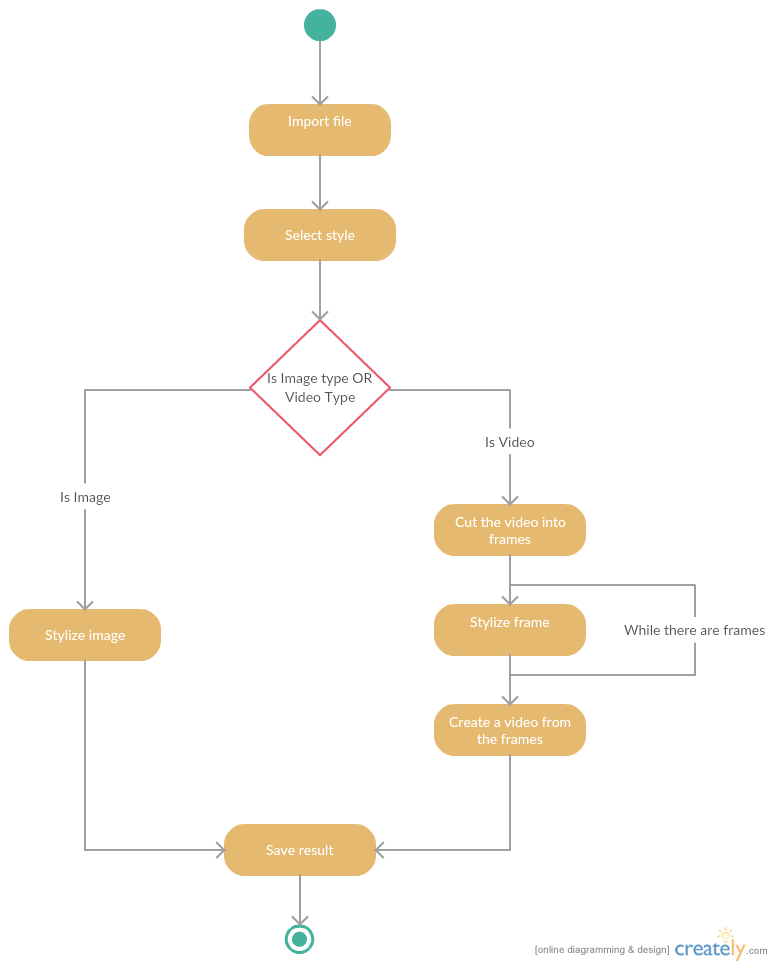
\includegraphics[scale=0.5]{software_overview.png}
		\caption{{A rendszer működése felülnézetből}}
		\label{felulnezet_1}
	\end{center}
\end{figure}

\section{A tanítási módszer állóképek esetében}
\secro{A tanítási módszer állóképek esetében}
\secen{A tanítási módszer állóképek esetében}

A rendszer tanításához állokép esetében két legalább képt bemenet szükséges, az eredeti kép amire át szeretnénk ruházni a stílust és a stílust tartalmazó kép, aminek a stílusát át szeretnénk ruházni. Mindkét bemenet esetében felírunk egy veszteség függvényt amik részei a végső nagy tanítási függvénynek.

\subsection{Az eredeti kép tanításának a veszteségi függvénye}
\ssecro{Az eredeti kép tanításának a veszteségi függvénye}
\ssecen{Az eredeti kép tanításának a veszteségi függvénye}
A mély neurálos hálók (Deep Neural Networks) azon típúsai amik a legeredményesebbek a képfeldolgozási feladatok elvégzésben a konvolúciós hálok. Mesterséges intelligencia területén a konvolúciós hálók olyan feed-forward típusú neuronhálók, amiket a biológiai elsődleges látókéregről mintáztak. A háló kifejezetten arra volt tervezve és kifejlesztve, hogy kétdimenziós formákat ismerjen fel. A háló alapértelmezetten több rétegből tevődik össze:

\begin{itemize}
	\item konvolúciós réteg: a konvolúciós hálók alapkövei. A réteg súlyai úgynevezett konvolúciós szűrők alkotják, amelyek a forward pass lépés során tanítva vannak. Ez a tanítás lépés úgy történik, hogy a szűrőt végigtoljuk a bemeneten és konvolúciónak nevezett műveletet végzünk. 
	\item pooling layer: arra használatos, hogy a bemeneti adathalmazt méretét leszűkítsük úgy hogy a halmaz adott értékein valamely matematikai műveletet végzünk (átlagszámolás, maximum számolás, minimum számolás). Erre azért van szükségünk, hogy növeljük a tanulás gyorsaságát, csökkentsük a számítások komplexitását megakadályozva ezzel az "overfitting" bekövetkezését.
	\item fully connected layer: minden bemenet mindem más bemenettel kapcsolatban áll.
\end{itemize}

A konvolúciós hálók súlyzókként konvolúciós szűrőket tartalmaznak. Ezek, tárgyfelisrmerés tanítása esetében, az adott bemeneti kép különböző tulajdonságait fogják tartalmazni. Annak függvényében, hogy a háló topológiájában egy adott réteg hol helyezkedik el, más tulajdonságokat fognak raktározni a szűrök. Az bemeneti réteghez közel álló alacsony szintű rétegek az adott kép pixelinformációit próbálják megjegyezni ezzel szemben a magasabb szinten levő rétegek szűrői különböző tárgyakat, formákat próbálnak megjegyezn\cite{27}\cite{28}. A hálók által tartalmazott információ vizualizálható azáltal, hogy rekonstruáljuk a bemeneti képet a súlyzók alapján. Alacsony rétegek esetében apró módósításokkal visszanyerhető az eredeti kép míg magasabb rétegek esetében objektumok, formák nyerhetők vissza.

Az eredi kép tanításához egy már előre betanított mély konvolúciós neuronhálót használunk fel. A háló tudományos kontextusban VGG-19 név alatt terjedt el amit Simonyan K. és  Zisserman A. vezetett be publikációjukban\cite{29} ahol még a "model E" nevet viselte. Ez a háló gép látás és tárgyfelismerés céljából volt bevezetve olyan eredményeket produkálva e téren amik az emberi látással versengenek. Rétegei és topologiájának részletes bemutatása a \cite{29} publikációban történik, valamint a \ref{vgg_19} figurán is látható. Fontos megjegyezni, hogy a háló rétegeiből használva volt a 16 konvolúciós réteg, valamint az 5 pooling réteg, a teljesen összekötött rétegek nem voltak használva.

\begin{figure}[h]
	\begin{center}
		\includegraphics[scale=0.3]{vgg19_cropped.png}
		\caption{VGG-19 háló topológiája\cite{30}}
		\label{vgg_19}
	\end{center}
\end{figure}

A választás azért esett erre az előre betanított hálóra, mivel Yaroslav N. és Roman N. kutatása alapján\cite{16} összehasonlítva a AlexNet, GoogLeNet VGG-16 és VGG-19 halókat, a VGG-19 használata során sikerült a leglátványosabb képeket készíteni.
\newline
\indent
A konvolúciós neuron háló minden rétege tartalmaz egy adott számú szűrőt, amik különbőző tulajdonságokat tartalmaznak a bementi képről. Ebből kifolyólag maga a bemenet kódolva van a szűrőkben. Egy \(N\) tulajdonságót tartalmazó réteg \(N\) szűrővel rendelkezik amelyek mérete \(M\). Maga a réteg kimenete lementhető egy \(N * M\) -es mátrixban. Egy adott réteg válasza egy bemeneti képre vizualizálható, ha gradient descent módszert alkalmazunk egy fehér zajt tartalmazó bemeneti képen. Tehát, legyen \(R^l\) egy adott az \(l\) haló válasza egy adott bemeneti képre. Legyen \(W^l\) ugyanaz ar \(l\) háló válasza egy adott fehér zajt tartalmazó bemeneti kép esetében. Akkor felírható a veszteség függvény mint:

\begin{equation}
L(\vec{x}, \vec{r}, l) = \frac{1}{2}\sum{R^l_{ij} - W^l_{ij}}
\end{equation}

Ahol \(\vec{x}\) a bemeneti képet jeleni, \(\vec{r}\) pedig azt a kimeneti képet jelenti amit a rendszer generál a rétegek tulajdonságaiból.
Mindez Tensorflow környezetben a következőképpen nézne ki:

\begin{lstlisting}[language=Python]
for layer_name in CONTENT_LAYER:
	content_loss += content_weight * (2 * tf.nn.l2_loss(
		all_layers[layer_name] - content_features[layer_name]) /
		content_features[layer_name].size)

content_loss /= len(CONTENT_LAYER)
return content_loss

\end{lstlisting}

A \(CONTENT\_LAYER\) tuple típusú ami tartalmazza azoknak a rétegeknek az azonosítóját amik részt vesznek a veszteség függvény kiszámításában. A \(content\_features\) valtozó egy lista, ez tartalmazza az összes réteg válaszát a bemeneti eredeti képre. A visszaküldött érték egy tensor típusú, egyik részét fogja képezni a végső optimalizálandó veszteségfüggvénynek. 


\subsection{Az stílus kép tanításának a veszteségi függvénye}
\ssecro{Az stílus kép tanításának a veszteségi függvénye}
\ssecen{Az stílus kép tanításának a veszteségi függvénye}

as

%----------------------------------------------------------------
\chapter{A rendszer tesztelése}
\capterro{Testarea sistemului}
\capteren{The testing of the system}

testing

%----------------------------------------------------------------
\chapter{Összefoglaló}
\capterro{Concluzie}
\capteren{Conclusion}

összefoglaló

% Ábrajegyzék
%---------------------------------
\newpage
 \listoffigures


% thebibliography
%---------------------------------
\newpage
\begin{thebibliography}{1}

\bibitem {1}
Krizhevsky, A., Sutskever, I., and Hinton, G. E. ImageNet classification with deep convolutional neural networks (2012)

\bibitem{2}
Zeiler, M. D. and Fergus, R. Visualizing and understanding convolutional networks (2013)

\bibitem{3}
\url {https://en.wikipedia.org/wiki/CUDA} (2017.04.24)

\bibitem{4}
\url {http://caffe.berkeleyvision.org} (2017.04.24)

\bibitem{5}
\url {https://keras.io/} (2017.04.24)

\bibitem{6}
\url {http://deeplearning.net/software/theano/} (2017.04.24)

\bibitem{7}
\url {https://www.tensorflow.org/} (2017.04.24)

\bibitem{8}
\url {http://torch.ch/} (2017.04.24)

\bibitem{9}
\url {https://computerstories.net/microsoft-computer-outperforms-human-image-recognition-12028} (2017.04.29)

\bibitem{10}
Kevin Alfianto, Mei-Chen Yeh, Kai-Lung Hua - Artist-based Classification via Deep Learning with Multi-scale Weighted Pooling (2016)

\bibitem{11}
Rosenblatt F. - The Perceptron: A Probabilistic Model For Information Storage And Organization In The Brain (1958)

\bibitem{12}
Werbos, P.J. - Beyond Regression: New Tools for Prediction and Analysis in the Behavioral Sciences (1975)
 
\bibitem{13}
LeCun, Yann, Léon Bottou, Yoshua Bengio, Patrick Haffner - Gradient-based learning applied to document recognition (1998)

\bibitem{14}
Dave Steinkraus, Patrice Simard. Ian Buck - Using GPUs for Machine Learning Algorithms (2005)

\bibitem{15}
Gatys, L. A., Ecker, A. S., Bethge - A neural algorithm of artistic style (2015)

\bibitem{16}
Yaroslav Nikulin, Roman Novak - Exploring the Neural Algorithm of Artistic Style (2016)

\bibitem{17}
Justin Johnson, Alexandre Alahi, Li Fei-Fei - Perceptual Losses for Real-Time Style Transfer and Super-Resolution

\bibitem{18}
Ulyanov, D., Lebedev, V., Vedaldi, A., and Lempitsky - Texture networks: Feed-forward synthesis of textures and stylized images

\bibitem{19}
Ulyanov, D., Lebedev, V., Vedaldi, A., and Lempitsky - Instance Normalization: The Missing Ingredient for Fast Stylization

\bibitem{20}
\url{https://en.wikipedia.org/wiki/Prisma_(app)} (2017.04.29)

\bibitem{21}
Manuel Ruder, Alexey Dosovitskiy, Thomas Brox - Artistic style transfer for videos (2016)

\bibitem{22}
asd

\bibitem{23}
\url{https://www.python.org/} (2017.04.30)

\bibitem{24}
\url{http://www.numpy.org/} (2017.04.30)

\bibitem{25}
\url{https://www.riverbankcomputing.com/software/pyqt/intro} (2017.04.30)

\bibitem{26}
\url{http://opencv.org/} (2017.04.30)

\bibitem{27}
Gatys, L. A., Ecker, A. S., Bethge, M. Texture synthesis and the controlled generation of natural stimuli using convolutional neural networks (2015)

\bibitem{28}
url{https://research.googleblog.com/2015/06/inceptionism-going-deeper-into-neural.html} (2017.05.01)

\bibitem{29}
Simonyan, K., Zisserman, A. - Very Deep Convolutional Networks for Large-Scale ImageRecognition (2015)

\bibitem{30}
http://dandxy89.github.io/ImageModels/vgg19/ (2017.05.01)


\end{thebibliography}

\end{document}
